\chapter{Modelo de dominio}
\label{cap:modelo}

El modelo representa los conceptos del servicio de pr\'estamos de la Escuela, sus relaciones y reglas. Es conceptual: orienta el esquema relacional, pero no prescribe todav\'ia tablas, interfaz o tecnolog\'ia de despliegue. Se distingue entre \textbf{tipo de bien} (por ejemplo, libro), \textbf{bien} (la ficha de un t\'itulo o modelo) y \textbf{unidad de inventario} (el ejemplar concreto que se presta).

\section{Entidades y conceptos principales}
\label{sec:entidades}

\subsection{Persona}
Representa a una persona natural vinculada a la Escuela, no a una empresa ni a un solicitante externo.

\textbf{Atributos:} identificador, documento de identidad, nombre completo, correo, contacto, estado activo o inactivo y fecha de registro.

\textbf{Reglas:} el documento es obligatorio y \'unico incluso si la persona est\'a inactiva. Se conserva un solo registro por persona para no fragmentar su historial. Una persona puede no tener cuenta todav\'ia. Desactivarla desactiva su cuenta e invalida sus sesiones, sin eliminar obligaciones pendientes.

\subsection{Usuario}
Representa la cuenta de acceso de una persona.

\textbf{Atributos:} identificador, persona, rol, nombre de usuario, hash de contrase\~na, estado y fecha del \'ultimo acceso.

\textbf{Reglas:} cada usuario pertenece a una persona; una persona tiene como m\'aximo una cuenta, activa o inactiva. El nombre de usuario es \'unico. Una cuenta activa exige una persona activa. La cuenta debe estar activa para solicitar o recibir bienes. Su desactivaci\'on no borra deudas, pr\'estamos ni sanciones.

\subsection{Rol y perfiles}
El rol define permisos y participa en la selecci\'on de pol\'iticas. Sus valores son administrador, docente y estudiante. Contiene identificador, nombre \'unico y descripci\'on.

\textbf{PerfilEstudiante:} usuario, c\'odigo universitario \'unico, programa, plan de estudios, semestre y habilitaci\'on vigente. El semestre debe pertenecer al plan, sin imponer arbitrariamente un rango de 1 a 12.

\textbf{PerfilDocente:} usuario, c\'odigo institucional \'unico, especialidad, vinculaci\'on con la Escuela y habilitaci\'on vigente.

Cada perfil pertenece a una cuenta. Un usuario puede tener como m\'aximo un perfil de cada tipo; el perfil correspondiente al rol actual es obligatorio y debe estar habilitado para prestar. Un perfil de un rol anterior puede conservarse como antecedente, pero no concede permisos adicionales. El administrador no requiere un perfil de solicitante.

\subsection{TipoBien}
Clasifica las fichas del cat\'alogo. Sus atributos son identificador, nombre \'unico y descripci\'on. Los valores permitidos en esta versi\'on son libro, mesa de ping-pong, visor 3D, parlante y carrito para rob\'otica. No incluye computadoras ni una categor\'ia de recursos de laboratorio.

\subsection{Bien}
Es la ficha descriptiva de un t\'itulo, modelo u objeto del cat\'alogo; no representa por s\'i sola una unidad prestable.

\textbf{Atributos comunes:} identificador, tipo de bien, nombre y descripci\'on.

\textbf{Datos seg\'un el tipo:} t\'itulo, autor, edici\'on e ISBN para libros; marca y modelo para dispositivos cuando corresponda. No se exige fabricante a un libro ni ISBN a un parlante. Estos datos podr\'an implementarse como atributos opcionales o fichas especializadas durante el dise\~no l\'ogico.

\textbf{Reglas:} cada bien pertenece a exactamente un tipo. El ISBN no identifica un ejemplar f\'isico y no sustituye al c\'odigo de inventario.

\subsection{UnidadInventario}
Es el ejemplar u objeto f\'isico concreto que puede entregarse o habilitarse para uso en sitio.

\textbf{Atributos:} identificador, bien, c\'odigo de inventario, adscripci\'on o custodia institucional, serie opcional, ubicaci\'on, condici\'on f\'isica, accesorios incluidos, estado (disponible, prestada, mantenimiento o baja), fecha de adquisici\'on opcional, fecha y motivo de baja opcionales y observaciones.

\textbf{Reglas:} el c\'odigo de inventario es obligatorio y \'unico. Solo se admite una unidad bajo custodia de la Escuela y no adscrita a laboratorios, independientemente de su tipo o ubicaci\'on. Si existe serie, se registra con marca y modelo y se evita duplicar esa combinaci\'on. Una unidad no puede tener m\'as de un pr\'estamo abierto. La disponibilidad para un intervalo combina su estado f\'isico con reservas y pr\'estamos; no es un simple campo booleano. Sus accesorios se controlan como parte de la entrega de esa unidad, no como pr\'estamos independientes en esta versi\'on.

\subsection{PoliticaPrestamo}
Es una versi\'on de las reglas autorizadas por la Escuela.

\textbf{Atributos:} identificador y versi\'on, rol opcional, tipo de bien opcional, inicio y fin de vigencia, responsable y fecha de aprobaci\'on, duraci\'on m\'axima y unidad de tiempo, modalidades permitidas, exigencia y tipos de garant\'ia, renovaci\'on permitida y cantidad m\'axima, tolerancia, tarifa diaria y reglas de bloqueo y liberaci\'on de garant\'ia. Las pol\'iticas generales o de rol incluyen adem\'as el l\'imite total de unidades simult\'aneas.

\textbf{Alcances admitidos:} general (sin rol ni tipo), por rol (rol definido y tipo vac\'io) y por rol y tipo (ambos definidos). No se admite tipo definido sin rol. Cada versi\'on contiene las condiciones de su alcance; la selecci\'on sigue RF-010.

\textbf{Reglas:} no se superponen vigencias de versiones de un mismo alcance. Las versiones utilizadas se conservan y no se reescriben. Una pol\'itica por tipo no modifica el cupo total por persona. No se asignan pol\'iticas de solicitante al rol administrador.

\subsection{Reserva}
Es una solicitud de uso anticipado de una unidad por parte de un estudiante o docente.

\textbf{Atributos:} identificador, usuario solicitante, unidad, creaci\'on, inicio y fin solicitados, estado, uso previsto, administrador que decide y fecha y motivo de la decisi\'on cuando corresponda.

\textbf{Reglas:} el fin es posterior al inicio. Solo una reserva confirmada bloquea el intervalo. Una reserva puede originar cero o un pr\'estamo y debe referirse al mismo usuario y unidad que este. Confirmar no garantiza la entrega si posteriormente aparecen retrasos, da\~nos, bloqueos u otras condiciones que la impidan; se revalida al entregar.

\subsection{Prestamo}
Es la operaci\'on central: asigna temporalmente la responsabilidad sobre una unidad a un solicitante.

\textbf{Atributos:} identificador, usuario solicitante, administrador que autoriza, unidad, reserva de origen opcional, estado, inicio, vencimiento inicial y vigente, devoluci\'on real opcional, cierre por p\'erdida opcional, modalidad de uso, condici\'on y accesorios de entrega y devoluci\'on, administrador que recibe o cierra y observaciones.

\textbf{Condiciones aplicadas:} conserva el rol de origen, las referencias a las versiones de pol\'itica usadas y una copia de los valores efectivos de plazo, cupo, garant\'ia, renovaci\'on, tolerancia, tarifa y bloqueo. Esta copia es un objeto de valor del pr\'estamo, no una pol\'itica editable. Un cambio posterior de rol o tarifa no modifica las condiciones ya acordadas.

\textbf{Reglas:} tiene exactamente un solicitante, una unidad y un administrador autorizante. El vencimiento es posterior al inicio. Los estados activo y vencido mantienen la responsabilidad y ocupan cupo; devuelto y cerrado por p\'erdida son terminales. Una operaci\'on rechazada antes de la entrega no crea un pr\'estamo abierto.

\subsection{Renovacion}
Registra una ampliaci\'on autorizada del plazo de un pr\'estamo existente.

\textbf{Atributos:} identificador, pr\'estamo, solicitante, administrador que autoriza, fecha de autorizaci\'on, vencimiento anterior, nuevo vencimiento y observaciones.

\textbf{Reglas:} el solicitante es el titular del pr\'estamo. La autorizaci\'on ocurre antes del vencimiento anterior y el nuevo vencimiento es posterior a este. Las renovaciones forman una secuencia coherente y no superan el n\'umero ni la duraci\'on permitidos. Su registro y la actualizaci\'on del pr\'estamo son at\'omicos.

\subsection{Garantia}
Representa un bien autorizado en custodia o un compromiso firmado para respaldar el pr\'estamo.

\textbf{Atributos:} identificador, pr\'estamo, tipo, naturaleza f\'isica o documental, descripci\'on o referencia, fecha y responsable de recepci\'on, estado (vigente, liberada o perdida), fecha y responsable de liberaci\'on opcionales y observaciones.

\textbf{Reglas:} un pr\'estamo tiene cero o una garant\'ia y exactamente una si su pol\'itica la exige. Solo una garant\'ia f\'isica puede declararse perdida; la incidencia asociada documenta su tratamiento. Liberar un compromiso no se describe como devolver un objeto. Los datos identificativos de la persona no constituyen autom\'aticamente una garant\'ia.

\subsection{Sancion}
Representa una consecuencia de un incumplimiento asociado a un pr\'estamo.

\textbf{Atributos:} identificador, pr\'estamo, usuario sancionado, tipo, motivo, fundamento de pol\'itica, monto, evidencia y fecha de pago opcionales, inicio y fin de bloqueo opcionales, suspensi\'on de bloqueo con motivo si corresponde, estado, fecha de registro, responsable (administrador o proceso autom\'atico) y datos de apelaci\'on y resoluci\'on.

\textbf{Reglas:} el sancionado es el solicitante del pr\'estamo. Monto y duraciones no son negativos; si hay bloqueo, su fin es posterior al inicio. Pago y cumplimiento temporal son obligaciones distintas. Un bloqueo impide nuevas reservas, entregas y renovaciones mientras su intervalo est\'e vigente y la sanci\'on no est\'e anulada ni tenga suspensi\'on registrada. Debe haber como m\'aximo una sanci\'on autom\'atica de retraso por pr\'estamo.

\subsection{Incidencia}
Representa una anomal\'ia ocurrida durante el pr\'estamo, la devoluci\'on o la custodia de su garant\'ia.

\textbf{Atributos:} identificador, pr\'estamo, garant\'ia relacionada opcional, tipo, descripci\'on, informante, administrador que registra, fecha, estado (abierta o resuelta), acci\'on correctiva y fecha y responsable de resoluci\'on opcionales.

\textbf{Reglas:} resolver exige documentar la acci\'on tomada. Si refiere una garant\'ia, esta debe pertenecer al mismo pr\'estamo. Puede existir una incidencia sin sanci\'on; por ejemplo, la p\'erdida de una garant\'ia bajo custodia de la Escuela no atribuye autom\'aticamente culpa al solicitante.

\subsection{EventoHistorial}
Es el registro de auditor\'ia de una operaci\'on significativa.

\textbf{Atributos:} identificador, usuario actor opcional, identificaci\'on del proceso autom\'atico si corresponde, entidad e identificador afectados, acci\'on, fecha y hora, resultado y detalle de cambios relevante para la trazabilidad.

\textbf{Reglas:} todo evento identifica un actor humano o un proceso; no queda an\'onimo. Es de solo adici\'on desde la aplicaci\'on. No almacena credenciales ni sustituye a las entidades de negocio. Las correcciones se expresan mediante nuevos eventos enlazados a los anteriores.

\section{Diagrama conceptual}
\label{sec:diagrama}

La figura~\ref{fig:dominio} muestra el n\'ucleo del dominio. Los extremos indican cu\'antas instancias pueden vincularse con una instancia del extremo opuesto. Se omiten perfiles, renovaciones, pol\'iticas e historial para mantener la legibilidad; sus relaciones se detallan en la tabla~\ref{tab:relaciones}.

\begin{figure}[htbp]
\centering
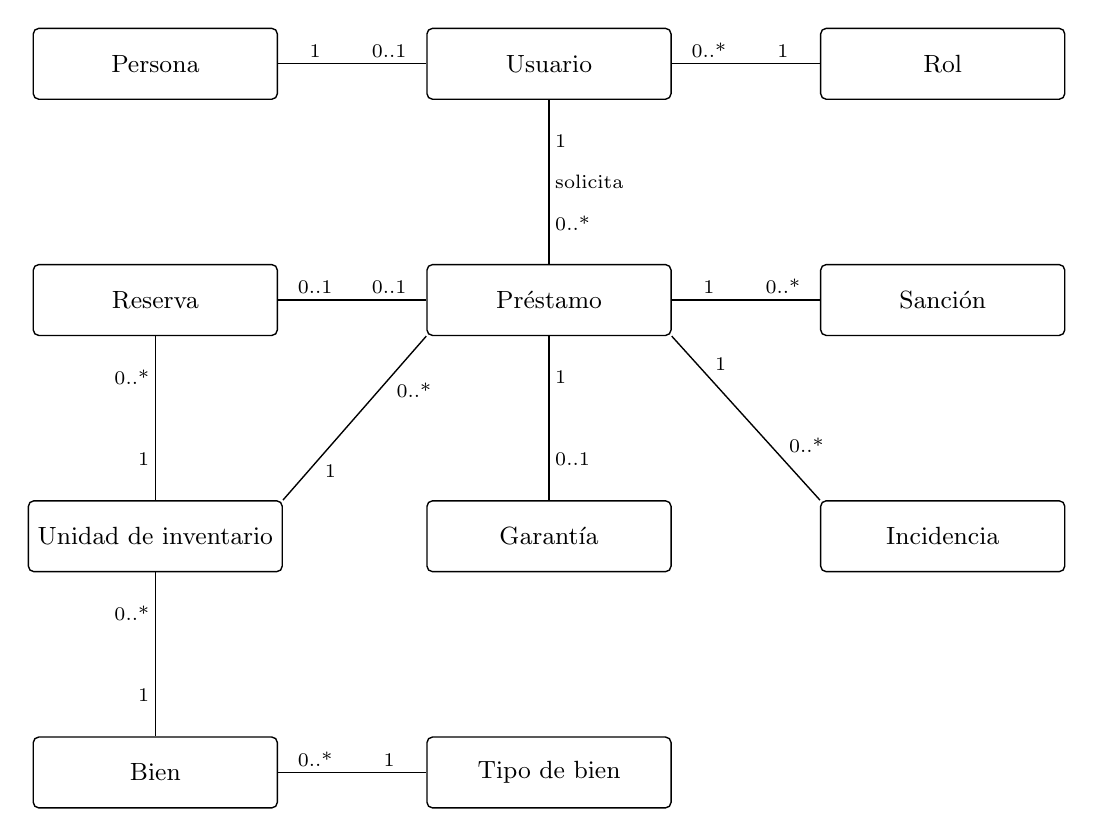
\begin{tikzpicture}[
    entidad/.style={draw,rounded corners=2pt,minimum width=3.1cm,minimum height=0.9cm,align=center,font=\small},
    cardinal/.style={font=\scriptsize,fill=white,inner sep=2pt},
    every path/.style={line width=0.5pt}
]
    \node[entidad] (persona) at (0,0) {Persona};
    \node[entidad] (usuario) at (5,0) {Usuario};
    \node[entidad] (rol) at (10,0) {Rol};
    \node[entidad] (reserva) at (0,-3) {Reserva};
    \node[entidad] (prestamo) at (5,-3) {Pr\'estamo};
    \node[entidad] (sancion) at (10,-3) {Sanci\'on};
    \node[entidad] (unidad) at (0,-6) {Unidad de inventario};
    \node[entidad] (garantia) at (5,-6) {Garant\'ia};
    \node[entidad] (incidencia) at (10,-6) {Incidencia};
    \node[entidad] (bien) at (0,-9) {Bien};
    \node[entidad] (tipo) at (5,-9) {Tipo de bien};

    \draw (persona) -- node[cardinal,near start,above]{1} node[cardinal,near end,above]{0..1} (usuario);
    \draw (usuario) -- node[cardinal,near start,above]{0..*} node[cardinal,near end,above]{1} (rol);
    \draw (usuario) -- node[cardinal,near start,right]{1} node[cardinal,midway,right]{solicita} node[cardinal,near end,right]{0..*} (prestamo);
    \draw (reserva) -- node[cardinal,near start,above]{0..1} node[cardinal,near end,above]{0..1} (prestamo);
    \draw (reserva) -- node[cardinal,near start,left]{0..*} node[cardinal,near end,left]{1} (unidad);
    \draw (unidad.north east) -- node[cardinal,near start,below right]{1} node[cardinal,near end,below right]{0..*} (prestamo.south west);
    \draw (prestamo) -- node[cardinal,near start,above]{1} node[cardinal,near end,above]{0..*} (sancion);
    \draw (prestamo) -- node[cardinal,near start,right]{1} node[cardinal,near end,right]{0..1} (garantia);
    \draw (prestamo.south east) -- node[cardinal,near start,above right]{1} node[cardinal,near end,above right]{0..*} (incidencia.north west);
    \draw (unidad) -- node[cardinal,near start,left]{0..*} node[cardinal,near end,left]{1} (bien);
    \draw (bien) -- node[cardinal,near start,above]{0..*} node[cardinal,near end,above]{1} (tipo);
\end{tikzpicture}
\caption{N\'ucleo del modelo de dominio de pr\'estamos}
\label{fig:dominio}
\end{figure}

\section{Cardinalidades y relaciones}

En la tabla, cada fila se lee desde una instancia de la entidad de origen. La multiplicidad \texttt{0..*} significa cero o muchas; \texttt{0..1}, opcional y como m\'aximo una. Las relaciones hist\'oricas no autorizan operaciones simult\'aneas incompatibles.

\begingroup
\small
\begin{longtable}{@{}>{\raggedright\arraybackslash}p{3.1cm}>{\raggedright\arraybackslash}p{3.2cm}>{\raggedright\arraybackslash}p{8cm}@{}}
\caption{Relaciones del modelo de dominio}\label{tab:relaciones}\\
\toprule
\textbf{Origen} & \textbf{Destino} & \textbf{Regla de asociaci\'on} \\
\midrule
\endfirsthead
\toprule
\textbf{Origen} & \textbf{Destino} & \textbf{Regla de asociaci\'on} \\
\midrule
\endhead
\bottomrule
\endfoot
Persona & Usuario & Una persona tiene 0..1 cuenta; cada cuenta pertenece a 1 persona. \\
Usuario & Rol & Cada usuario tiene 1 rol; un rol clasifica 0..* usuarios. \\
Usuario & Perfil & Tiene 0..1 perfil de cada tipo; el del rol solicitante actual es obligatorio. Cada perfil pertenece a 1 usuario. \\
TipoBien & Bien & Un tipo agrupa 0..* fichas; cada ficha tiene 1 tipo. \\
Bien & UnidadInventario & Una ficha describe 0..* unidades; cada unidad corresponde a 1 ficha. \\
Rol / TipoBien & PoliticaPrestamo & Cada rol o tipo puede participar en 0..* versiones; una versi\'on refiere 0..1 rol y 0..1 tipo seg\'un su alcance. \\
Usuario & Reserva & Un solicitante tiene 0..* reservas; cada reserva tiene 1 solicitante. \\
UnidadInventario & Reserva & Una unidad tiene 0..* reservas hist\'oricas; cada reserva corresponde a 1 unidad. \\
Reserva & Prestamo & Una reserva origina 0..1 pr\'estamo; un pr\'estamo procede de 0..1 reserva. No es una relaci\'on de una reserva con varios pr\'estamos. \\
Usuario & Prestamo & Como solicitante, tiene 0..* pr\'estamos; cada pr\'estamo tiene 1 solicitante. Como administrador, autoriza 0..* entregas; cada pr\'estamo tiene 1 autorizante. \\
UnidadInventario & Prestamo & Una unidad registra 0..* pr\'estamos hist\'oricos, pero como m\'aximo 1 abierto; cada pr\'estamo tiene 1 unidad. \\
Prestamo & PoliticaPrestamo & Conserva referencias a las versiones que aportan condiciones y cupo; una versi\'on puede respaldar 0..* pr\'estamos. \\
Prestamo & Renovacion & Tiene 0..* renovaciones; cada renovaci\'on pertenece a 1 pr\'estamo y tiene 1 administrador autorizante. \\
Prestamo & Garantia & Tiene 0..1 garant\'ia, obligatoria si se exige; cada garant\'ia pertenece a 1 pr\'estamo. \\
Prestamo & Sancion & Puede originar 0..* sanciones; cada sanci\'on refiere 1 pr\'estamo y a su solicitante. \\
Prestamo & Incidencia & Tiene 0..* incidencias; cada incidencia pertenece a 1 pr\'estamo. \\
Garantia & Incidencia & Puede tener 0..* incidencias; una incidencia refiere 0..1 garant\'ia del mismo pr\'estamo. \\
Usuario & EventoHistorial & Un usuario genera 0..* eventos; cada evento tiene 0..1 usuario actor, obligatorio salvo que se identifique un proceso autom\'atico. \\
\end{longtable}
\endgroup

\section{Ciclos de vida}
\label{sec:estados}

\subsection{Reserva}
\begin{itemize}
    \item Pendiente: solicitud registrada sin bloqueo de disponibilidad.
    \item Confirmada: solicitud aprobada; el intervalo queda comprometido para la unidad y el solicitante.
    \item Rechazada: solicitud pendiente denegada con motivo.
    \item Cancelada: solicitud pendiente o confirmada retirada antes de la entrega.
    \item Atendida: reserva confirmada convertida en su \'unico pr\'estamo.
    \item Vencida: reserva pendiente o confirmada cuyo intervalo termin\'o sin entrega.
\end{itemize}

Las transiciones permitidas son pendiente a confirmada, rechazada, cancelada o vencida, y confirmada a atendida, cancelada o vencida. Los estados terminales no se reabren; una nueva solicitud genera otra reserva. El paso a vencida debe efectuarse antes de evaluar operaciones que dependan de su vigencia, aunque no exista un proceso peri\'odico en ejecuci\'on.

\subsection{Pr\'estamo}
\begin{itemize}
    \item Activo: entrega registrada, sin devoluci\'on ni cierre y con plazo a\'un no superado.
    \item Vencido: sigue abierto y la fecha y hora actuales superan el vencimiento vigente.
    \item Devuelto: se registr\'o la recepci\'on e inspecci\'on del bien.
    \item Cerrado por p\'erdida: el administrador document\'o la imposibilidad de devoluci\'on y dio de baja la unidad.
\end{itemize}

Las transiciones son activo a vencido, devuelto o cerrado por p\'erdida, y vencido a devuelto o cerrado por p\'erdida. Una renovaci\'on v\'alida mantiene el estado activo y cambia el vencimiento; no permite reactivar un pr\'estamo ya vencido. El estado vencido debe derivarse del reloj y del cierre, o actualizarse de forma consistente antes de cada consulta u operaci\'on. No puede depender de una tarea manual.

\subsection{Unidad y obligaciones asociadas}
La entrega cambia la unidad de disponible a prestada en la misma transacci\'on que crea el pr\'estamo. Mientras este est\'a activo o vencido, la unidad permanece prestada. La devoluci\'on la lleva a disponible, mantenimiento o baja seg\'un la inspecci\'on; el cierre por p\'erdida la lleva a baja. Una unidad en mantenimiento puede volver a disponible tras verificaci\'on administrativa. Una baja es terminal dentro de esta versi\'on.

Cerrar el pr\'estamo no equivale a liberar toda obligaci\'on: las garant\'ias, incidencias y sanciones conservan sus propios estados hasta su resoluci\'on. Se permite registrar esa resoluci\'on aunque la cuenta del titular est\'e inactiva.

\section{Reglas de integridad}
\label{sec:integridad}

\subsection{Identidad y referencias}
\begin{itemize}
    \item Son \'unicos el documento de persona, nombre de usuario, referencia de persona en la cuenta, c\'odigos de perfiles, nombre de tipo de bien y c\'odigo de inventario.
    \item La referencia a reserva en un pr\'estamo es opcional y \'unica cuando existe; la referencia a pr\'estamo en una garant\'ia es obligatoria y \'unica.
    \item La serie no es obligatoria para todos los bienes. Se controla la combinaci\'on marca, modelo y serie cuando se registra; el ISBN puede compartirse entre ejemplares.
    \item Solicitante, unidad, autorizante, inicio, vencimiento y condiciones aplicadas son obligatorios en todo pr\'estamo.
    \item Las referencias hist\'oricas se conservan mediante desactivaci\'on o baja l\'ogica; no se eliminan en cascada pr\'estamos, garant\'ias, sanciones o eventos.
\end{itemize}

\subsection{Tiempo, disponibilidad y cupo}
Dos intervalos $[i_1,f_1)$ y $[i_2,f_2)$ se solapan si y solo si:
\[
    i_1 < f_2 \quad \land \quad i_2 < f_1.
\]

\begin{itemize}
    \item Toda reserva tiene fin posterior a inicio. Todo pr\'estamo tiene vencimiento posterior a entrega. Devoluci\'on y cierre por p\'erdida, cuando existan, no pueden ser anteriores a la entrega y son mutuamente excluyentes.
    \item Un pr\'estamo devuelto exige fecha de devoluci\'on; uno cerrado por p\'erdida exige fecha de cierre e incidencia. Los abiertos no tienen ninguna de esas fechas.
    \item No se permiten reservas confirmadas solapadas para una unidad. Un pr\'estamo o renovaci\'on no puede invadir otra reserva confirmada; la reserva de origen se excluye al convertirla, para no contar dos veces la misma asignaci\'on.
    \item Un pr\'estamo abierto ocupa su intervalo hasta el vencimiento previsto para la planificaci\'on. Si ya est\'a vencido, la disponibilidad futura se considera bloqueada hasta la devoluci\'on o cierre efectivo. Nunca se entrega otra vez una unidad todav\'ia prestada.
    \item El cupo simult\'aneo se valida sobre todas las unidades del solicitante, no por cada tipo de manera independiente. Para intervalos futuros se suman las reservas confirmadas y los pr\'estamos abiertos que los intersectan; los vencidos se consideran abiertos sin fin conocido.
    \item La confirmaci\'on de reservas, las entregas y las renovaciones verifican tanto conflictos de unidad como de cupo dentro de la misma transacci\'on. Una consulta previa de disponibilidad no reemplaza esta verificaci\'on.
    \item Duraciones y cupos son positivos; tolerancia, tarifa, monto y n\'umero de renovaciones son no negativos. Si no se permiten renovaciones, su m\'aximo es cero.
\end{itemize}

\subsection{Garant\'ias, sanciones y auditor\'ia}
\begin{itemize}
    \item Una entrega que exige garant\'ia no puede confirmarse sin registrarla como vigente. La liberaci\'on exige fecha y responsable; una p\'erdida exige una incidencia vinculada.
    \item El usuario sancionado debe coincidir con el solicitante del pr\'estamo, nunca con el administrador que lo autoriz\'o por el solo hecho de autorizarlo.
    \item El c\'alculo autom\'atico de retraso es idempotente: repetir el procesamiento no duplica sanciones. Emplea la tarifa y tolerancia conservadas, y el vencimiento vigente.
    \item Una sanci\'on no se marca cumplida mientras quede una obligaci\'on econ\'omica o temporal pendiente. Una apelaci\'on y su resoluci\'on no borran el registro original.
    \item Los cambios de estado y sus eventos se confirman juntos. Un fallo no puede dejar un pr\'estamo creado sin ocupar la unidad, una reserva atendida sin pr\'estamo o una garant\'ia sin asociaci\'on.
\end{itemize}

La implementaci\'on deber\'a combinar restricciones declarativas, \'indices y validaciones transaccionales. Una restricci\'on sobre una sola fila no basta para impedir todos los solapamientos ni excesos de cupo.

